\documentclass{article}
\usepackage[utf8]{inputenc}
\usepackage[backend=biber]{biblatex}
\usepackage{amssymb}
\usepackage{amsmath}
\usepackage{dsfont}
\addbibresource{bib.bib}
\setlength{\parindent}{0em}
\bibliography{bib}
\setlength{\parskip}{6pt}
\usepackage[margin=1.0in]{geometry}
\usepackage{graphicx}
\usepackage{caption}
\usepackage{subcaption}
\usepackage{wrapfig}
\usepackage{url}

\title{Intro to deep learning with PyTorch}
\author{Miguel A. Saavedra-Ruiz}
\date{Abril 2020}
\linespread{1.0}

\nocite{*}


\begin{document}

\maketitle

\section{Introduction to Neural Networks}

Deep learning is everywhere, applications in games such as Go or jeopardy, detecting spam in emails, forecasting stock prices, recognizing images in a picture, and diagnosing illnesses sometimes with more precision than doctors are just few examples.

The heart of Deep learning are object called \textbf{neural networks}. Neural networks vaguely mimic the process of how the brain operates, with neurons that fire bits of information. The next image shows a neural network \ref{fig:f1}.

\begin{figure}[ht]
    \centering
    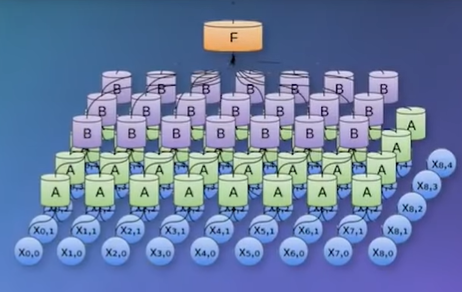
\includegraphics[width=0.35\textwidth,height=0.35\textheight,keepaspectratio]{images/nn.PNG}
    \captionsetup{justification=centering}
    \caption{A Neural network}
    \label{fig:f1}
\end{figure}

A neural network is a function approximator which is capable to split data. Given some data in the form of blue or red points, the neural network will look for the best line that separates the data \ref{fig:f2}..

\begin{figure}[ht]
    \centering
    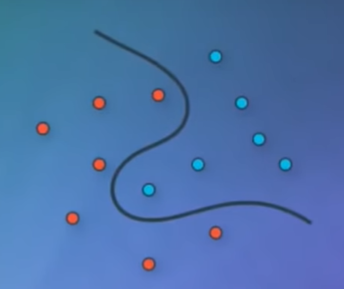
\includegraphics[width=0.2\textwidth,height=0.2\textheight,keepaspectratio]{images/data.PNG}
    \captionsetup{justification=centering}
    \caption{A Neural network splitting data}
    \label{fig:f2}
\end{figure}

The separation line is called a model and its job is to split the data. A model might not be perfect, but it most be as accurate as possible. Imagine the next example where we plot the acceptance rate of students based on their grades and test scores. The blue dots are accepted and red rejected. Furthermore, the line plotted is "the model" Fig. \ref{fig:f3}.

\begin{figure}[ht]
    \centering
    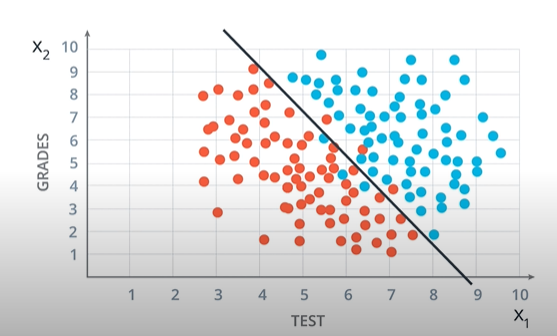
\includegraphics[width=0.5\textwidth,height=0.5\textheight,keepaspectratio]{images/example_1.PNG}
    \captionsetup{justification=centering}
    \caption{Neural network model}
    \label{fig:f3}
\end{figure}

Based on that, it is safe to predict that if a point is over the line the student gets accepted and if it's under the line then the student gets rejected.

Taking into account that Test is label as \(x_1\) and Grades as \(x_2\), the \textbf{boundary line} that separates the blue and the red points is going to have a linear equation. The equation of the one drawn above is describes in \eqref{eq:1}.

\begin{equation}
2 x_1 + x_2 - 18 = 0 \label{eq:1}
\end{equation}

The equation \eqref{eq:1} means that the method for accepting or rejecting students says the following: take this equation as our score where \(score =2.Test + Grades - 18\), if a student has \(score > 0\) the he gets accepted, otherwise he is rejected. This process is called a prediction. Additionally, by convention it is possible to say that if the score is 0, the student will get accepted although this won't matter much at the end. \textbf{The linear equation is out model}.

In the more general case, a boundary will be an equation of the following form \eqref{eq:2}.

\begin{equation}
wx_1+w_2x_2+b=0 \label{eq:2}
\end{equation}  

The last equation can be abbreviate in vector notation as \eqref{eq:3}.

\begin{equation}
wx+b=0 \label{eq:3}
\end{equation}  

Where w and x are vectors as shown below:

\[ w = (w_1, w_2)\]
\[ x = (x_1, x_2)\]

X can be refereed as the input, w as the weights and b as the bias. For a student coordinates \(x_1, x_2\), a label denoted as Y will be used as the value to predict. So if the student gets accepted, namely the point is blue,
then the label is \( y = 1\), And if the student gets rejected, namely the point is red and then the label is \( y = 0\)

The prediction made by our algorithm is going to be called \(\hat{y}\) and it will be what the algorithm predicts that the label will be \eqref{eq:4}. Where one means accepted and zero rejected.

\begin{equation}
\label{eq:4}
\hat{y} =
  \begin{cases}
    1, & \text{if } Wx + b \geq 0 \\
    0, & \text{if } Wx + b < 0 \\
  \end{cases}
\end{equation}  

So, to summarize, the points above the line have \( \hat{y} = 1\) and the points below the line have \( \hat{y} = 0\). And, the blue points have \( y = 1\) and the red points have \( y = 0\).

Subsequently, if we have more data columns so not just testing grades, but maybe something else like the ranking of the student in the class it will turn the problem into a three-dimensional space. The only difference now is that the problem won't be working in two dimensions but three. So now, the three axis are: \(x_1\) for the test, \(x_2\) for the grades and \(x_3\) for the class ranking. The data will looks like Fig. \ref{fig:f4}.

\begin{figure}[ht]
    \centering
    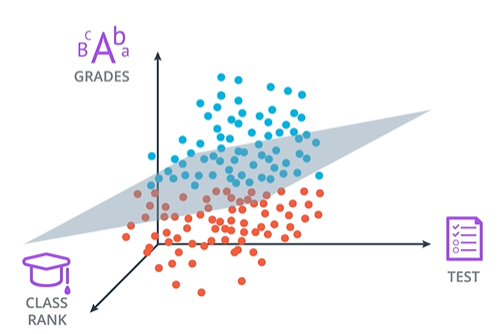
\includegraphics[width=0.5\textwidth,height=0.5\textheight,keepaspectratio]{images/example_2.PNG}
    \captionsetup{justification=centering}
    \caption{3D data example}
    \label{fig:f4}
\end{figure}

The equation won't be a line in two dimension, but a plane in three dimensions with a similar equation as before. Now, the equation would be \eqref{eq:5} which will separate this space into two regions.

\begin{equation}
w_1x_1 + w_2x_2 + w_3x_3 + b = 0, \label{eq:5}
\end{equation}  

This equation \eqref{eq:5} can still be abbreviated by \eqref{eq:3} (\(wx+b=0\)) except our vectors will now have three entries instead of two. The prediction will be the same as described by \eqref{eq:4}.

If we have many columns like say n of them as shown in Fig. \ref{fig:f5}, the data just leaps in n-dimensional space. Here the points are just things with n coordinates called \(x_1, x_2, x_3, \dots, x_n  \) with the labels being \(y\).

\begin{figure}[ht]
    \centering
    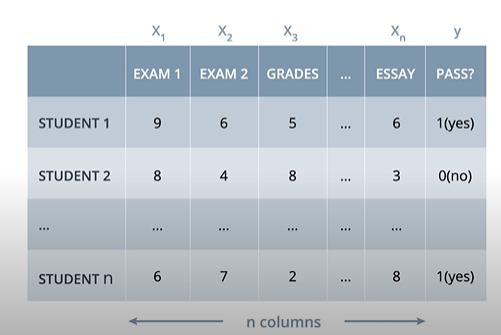
\includegraphics[width=0.5\textwidth,height=0.5\textheight,keepaspectratio]{images/multiple_dimension.PNG}
    \captionsetup{justification=centering}
    \caption{Multi-dimensional data}
    \label{fig:f5}
\end{figure}

Therefore, the boundaries just an \(n-1\) dimensional hyperplane, and the equation of this \(n-1\) dimensional hyperplane is going to be the one shown in \eqref{eq:6} or the abbreviated form shown in \eqref{eq:3} and the predictions still being the same as shown by equation \eqref{eq:4}.

\begin{equation}
w_1x_1 + w_2x_2 + \dots + w_n x_n + b = zero, \label{eq:6}
\end{equation}  

e.g Given the table in the Fig. \ref{fig:f5}, the dimensions for input features (x), the weights (W), and the bias (b) to satisfy (Wx + b) would be \( W(1xn), x(nx1) \text{and} b(1x1)\) for a single student.

Now it is time to introduce the notion of a \textbf{Perceptron}, which is the building block of neural networks. It is possible to show an example based on Fig. \ref{fig:f3}, where it is possible to encode the previous equations into a small graph. Let's fit The data and boundary line inside a node. Add small nodes for the inputs which in this case, they are the test and grades. The Fig. \ref{fig:f6} presents the mention before, with a specific value of test and grades. The Perceptron checks if the point is in the positive or negative area. If the point is in the positive area, then it returns a yes, otherwise a no.

\begin{figure}[ht]
    \centering
    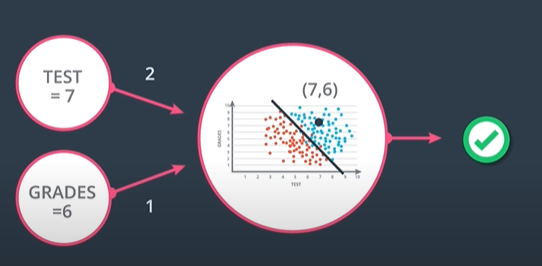
\includegraphics[width=0.5\textwidth,height=0.5\textheight,keepaspectratio]{images/perceptron_1.PNG}
    \captionsetup{justification=centering}
    \caption{Perceptron example with student admission}
    \label{fig:f6}
\end{figure}

Recall that the prediction consists of accepting the student based on \(score =2.Test + Grades - 18\), if the \( score \geq 0\) he gets accepted, and rejecting them if the \(score < 0\)

The weights \(2\), \(1\) and \(-18\) are what define the linear equation, and so they are used as labels in the graph Fig. \ref{fig:f6}. Another way to graph this node is to consider the bias as part of the input.

Since \(w_1\) gets multiplied by \(x_1\) and \(w_2\) by \(x_2\), it's natural to think that \(b\) gets multiplied by a one. So the bias will have the B labeling and and edge coming from a one. Then what the node does is it multiplies the values coming from the incoming nodes by the values and the corresponding edges. Then it adds them and finally, it checks if the result is greater than or equal to zero. If it is, then the node returns a yes or a value of one, and if it isn't then the node returns a no or a value of zero as shown in Fig. \ref{fig:f7}.

\begin{figure}[ht]
    \centering
    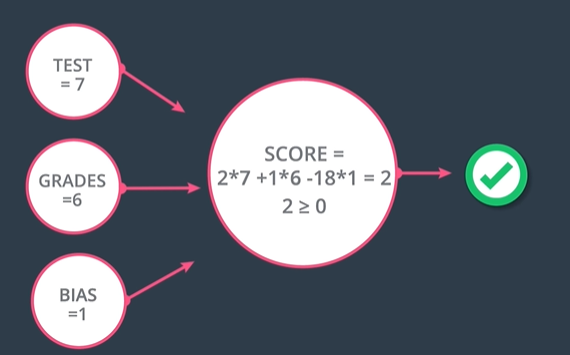
\includegraphics[width=0.45\textwidth,height=0.45\textheight,keepaspectratio]{images/perceptron_2.PNG}
    \captionsetup{justification=centering}
    \caption{Perceptron with weights and bias}
    \label{fig:f7}
\end{figure}

In the general case, a node looks like the one presented in Fig. \ref{fig:f8}.The node has inputs coming in with values \(x_1\) up to \(x_n\) and one (for the bias), and edges with weights \(w_1\) up to \(w_n\), and \(b\) corresponding to the bias unit. Then the node calculates the linear equation \eqref{eq:3}, which is this case is \(\sum_{i=1}^n w_i x_i + B\). This node then checks if the value is zero or bigger, and if it is, then the node returns a value of one for yes and if not, then it returns a value of zero for no. 

\[wx+b = \sum_{i=1}^n w_i x_i + b\]

\begin{figure}[ht]
    \centering
    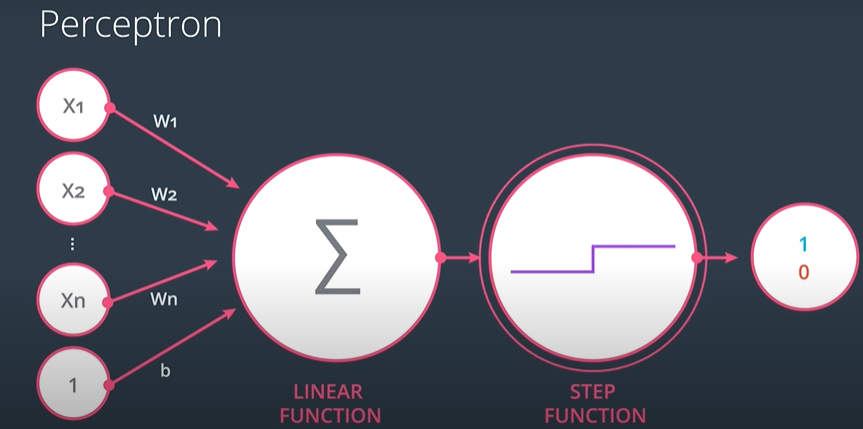
\includegraphics[width=0.5\textwidth,height=0.5\textheight,keepaspectratio]{images/general_perceptron.PNG}
    \captionsetup{justification=centering}
    \caption{General Perceptron}
    \label{fig:f8}
\end{figure}

In the last Figure, an implicit function is being used, this is called a step function. What the step function does is it returns a one if the input is positive or zero if the input is negative Fig. \ref{fig:f9}.

\begin{figure}[ht]
    \centering
    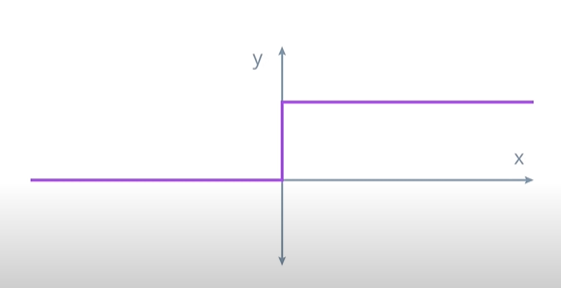
\includegraphics[width=0.4\textwidth,height=0.4\textheight,keepaspectratio]{images/step.PNG}
    \captionsetup{justification=centering}
    \caption{Step function}
    \label{fig:f9}
\end{figure}

\[
y =
  \begin{cases}
    1, & \text{if } x \geq 0 \\
    0, & \text{if } x < 0 \\
  \end{cases}
\]

In reality, the perceptron can be seen as a combination of nodes, where the first node calculates a linear equation based on the inputs and weights. The second node applies the step function to the result, giving the final outcome of the perceptron Fig. \ref{fig:f10}. The \(\sum\) represents a linear function in the first node and the drawing represents a step function in the second node. Nevertheless, we can use different step functions or generally, activation functions in this node.

\begin{figure}[ht]
    \centering
    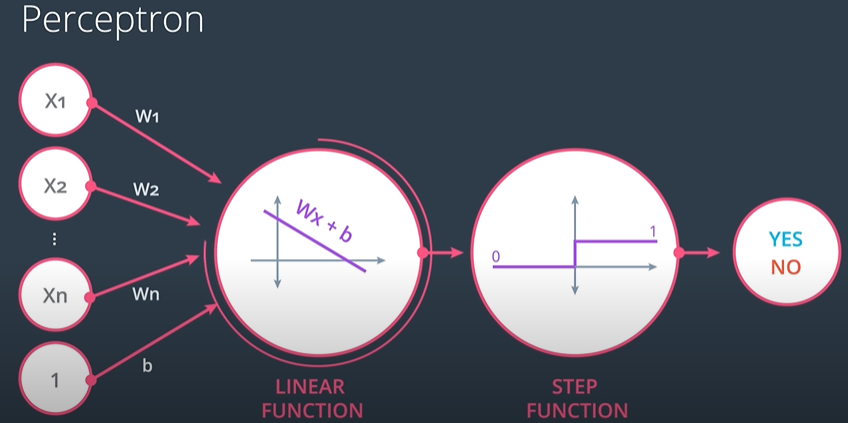
\includegraphics[width=0.5\textwidth,height=0.5\textheight,keepaspectratio]{images/simple_perceptron.PNG}
    \captionsetup{justification=centering}
    \caption{The simple perceptron}
    \label{fig:f10}
\end{figure}

The name "neural network" comes from the fact that perceptrons look like neurons in the brain. In the Fig. \ref{fig:f11} can be seen a perceptron in the Left with four inputs, these inputs are the dendrites in a Neuron and they receive nervous impulses. Similarly, the computation is made in the node of the perceptron or nucleus. Finally, the perceptron outputs the final result as a neuron does through its axon, which is the mechanism a neuron use to outputs nervous impulses. \textbf{The neural networks mimic the concept of neuron and brain} by taking the output from one neuron and turning it into the input for another one.

\begin{figure}[ht]
    \centering
    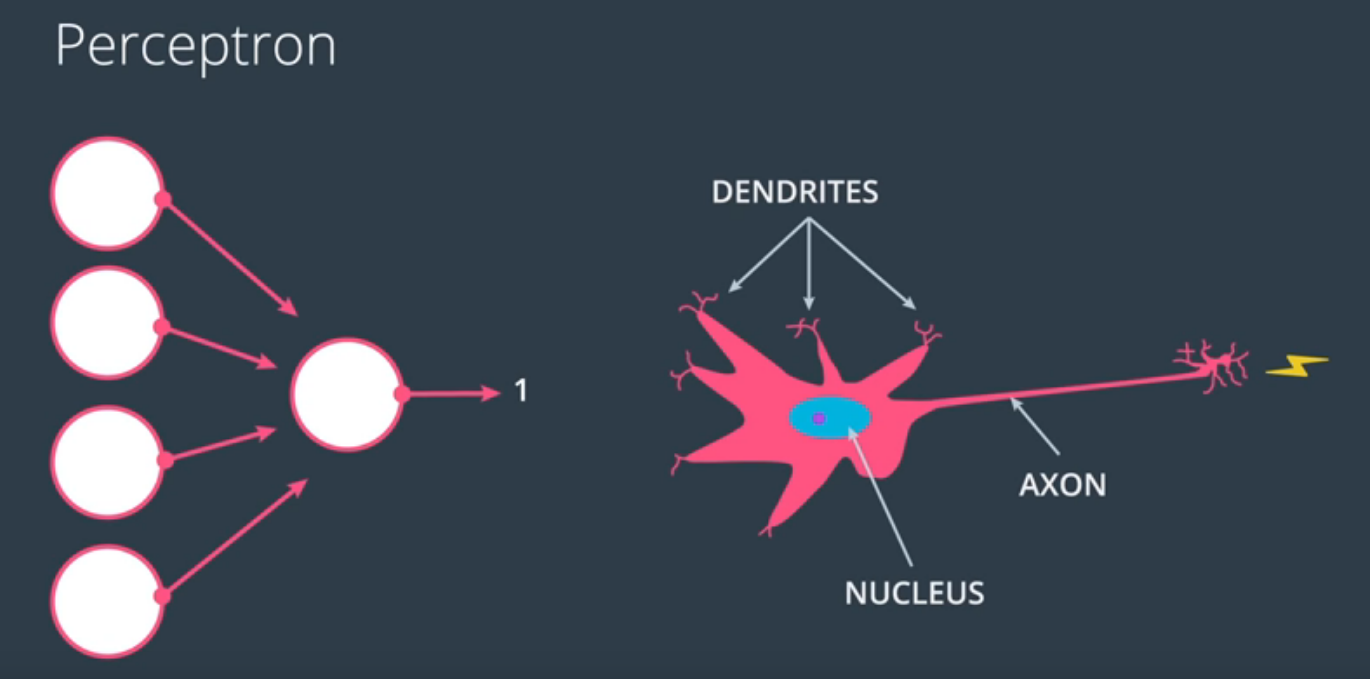
\includegraphics[width=0.5\textwidth,height=0.5\textheight,keepaspectratio]{images/perceotron_neuron.png}
    \captionsetup{justification=centering}
    \caption{The perceptron as a neuron}
    \label{fig:f11}
\end{figure}

Perceptrons can be used as logic operators (AND, OR, XOR). E.g the ND operator can be represented as a two inputs perceptron with 1 output, where the inputs can be 1 or 0 as well as the output. To recall the true table of the perceptron, it is presented in Fig. \ref{fig:f12}. The perceptron presented in the same figure shows how it splits the points with a boundary line, where the dots in the red area corresponds to a zero and the point in the blue area corresponds to a one. In the file called \textit{introduction/and\_perceptron.py} can be seen an example of this which use the general equation of a boundary \eqref{eq:2} (\(wx_1+w_2x_2+b=0\)). 

\begin{figure}[ht]
    \centering
    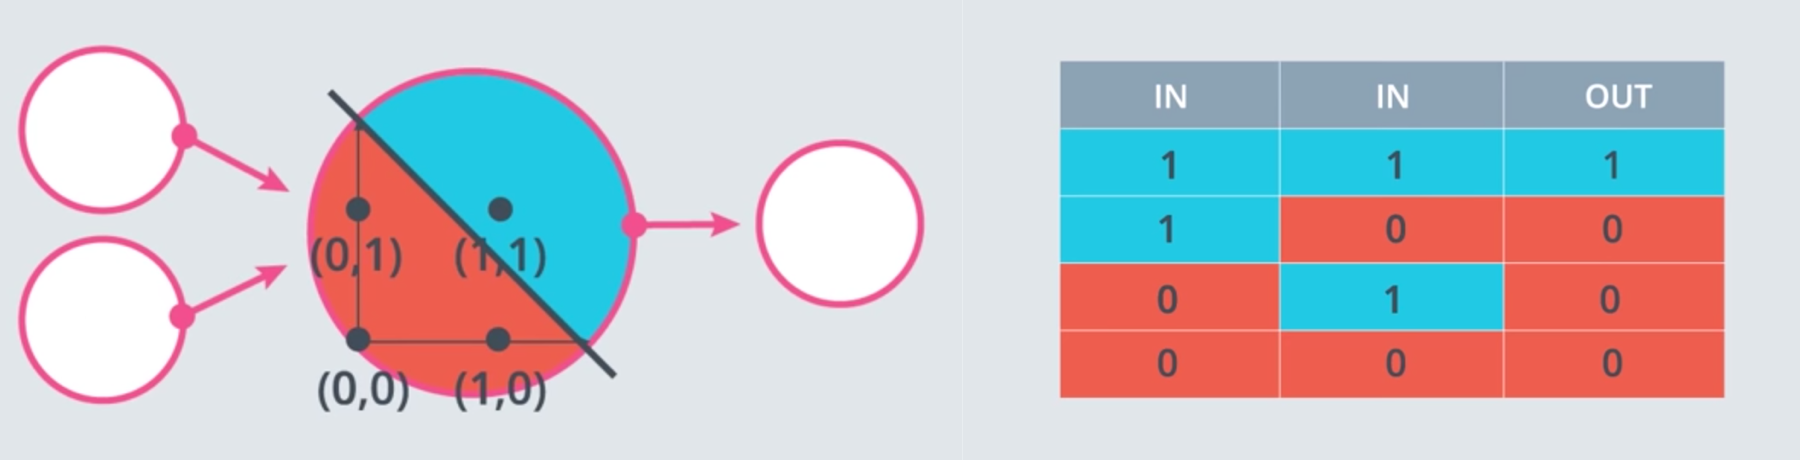
\includegraphics[width=0.5\textwidth,height=0.5\textheight,keepaspectratio]{images/and_table.png}
    \captionsetup{justification=centering}
    \caption{True table of the AND operator}
    \label{fig:f12}
\end{figure}

It is possible to represent logic operators as AND or OR with simple perceptrons, nevertheless, a problem arises when the problem has non-linear boundaries. 

To find the boundary line for a simple logic operator the process is really straightforward. Imagine a classification problem as shown by Fig. \ref{fig:f13}, the goal is to classify both the blue and red points correctly. However, there are one blue point and red point misclassified. To solve this, one logic approach would be to make the line closer to the misclassified points (located in the blue region) and hence change its label.

\begin{figure}[ht]
    \centering
    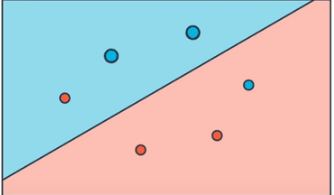
\includegraphics[width=0.25\textwidth,height=0.25\textheight,keepaspectratio]{images/split_data.png}
    \captionsetup{justification=centering}
    \caption{Splitting the data example}
    \label{fig:f13}
\end{figure}

Now imagine the line plotted in Fig. \ref{fig:f14}, where the line equation is given by \(3x_1+ 4x_2 - 10 = 0\) and out labels are: blue area if \(\hat{y} > 0\) or red area if \(\hat{y} < 0\). Suppose that the line has coordinates \((4,5)\), based on the approach described above, the point coordinates should be subtracted to the line equation as shown by the equation below, where \(x_1 = 4, x_2 = 5 \text{ and } b = 1\).

\[
\begin{bmatrix}  \text{new } w_1 \\
                 \text{new } w_2 \\
                \text{new } b \end{bmatrix} = \begin{bmatrix}
                                    3 - 4 \\
                                    4 - 5 \\
                                    -10 - 1
                                    \end{bmatrix} = \begin{bmatrix}
                                                    -1 \\
                                                    -1 \\
                                                    -11
                                                    \end{bmatrix}
\]

\begin{figure}[ht]
    \centering
    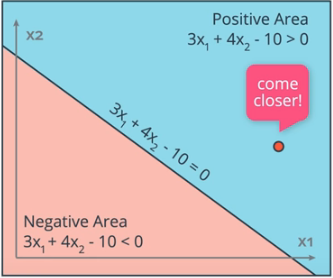
\includegraphics[width=0.25\textwidth,height=0.25\textheight,keepaspectratio]{images/moving_line.png}
    \captionsetup{justification=centering}
    \caption{Making the line closer example}
    \label{fig:f14}
\end{figure}

With the new parameters, the equation will be \(-1x_1+ 4-1x_2 - 11 = 0\). Nevertheless, this might be a very drastic change in the equation, leading to misclassification of other well-classified points. The idea is to make the line take small moves towards the misclassified point. To solve this, it is neccesary to take small steps towards the point, therefore, a new concept needs to be introduced. This concepts is called \(\alpha\) or \textbf{learning rate}. The learning rate is a small number between zero and one and its function is to minimize the change in the model equation by multiplying its value to the values of the point. E.g, using a learning rate of \(0.1\) and the same example as before, the result will be the shown in the equation and Fig. \ref{fig:f15}

\[
\begin{bmatrix}  \text{new } w_1 \\
                 \text{new } w_2 \\
                \text{new } b \end{bmatrix} = \begin{bmatrix}
                                    3 - 4*(0.1) \\
                                    4 - 5*(0.1) \\
                                    -10 - 1*(0.1)
                                    \end{bmatrix} = \begin{bmatrix}
                                                    2.6 \\
                                                    3.5 \\
                                                    -10.1
                                                    \end{bmatrix}
\]

\begin{figure}[ht]
    \centering
    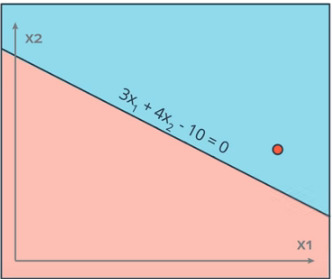
\includegraphics[width=0.25\textwidth,height=0.25\textheight,keepaspectratio]{images/new_line.png}
    \captionsetup{justification=centering}
    \caption{Moving the line closer to the point}
    \label{fig:f15}
\end{figure}

Similarly, if the misclassified point is located in the red area, instead of subtracting the point to the model equation it needs to be added. As a thumb rule, the \eqref{eq:7} shows the process of adding or substracting based on the point's location.

\begin{equation}
\label{eq:7}
  \begin{cases}
    Substract, & \text{if } \text{point is located in region } > 0 \\
    Add, & \text{if } \text{point is located in region } < 0 \\
  \end{cases}
\end{equation}  

Based on the technique given above, it is possible to determine the perceptron algorithm. This one is presented in the Fig. \ref{fig:f16} and shows and iterative process that tries to classify correctly all the misclassified points. The process works iteratively and can run until all the points are correctly classified or a minimum of misclassified points are obtained. A code example of this is given in \textit{introduction/perceptron\_algorithm.py}
  
\begin{figure}[ht]
    \centering
    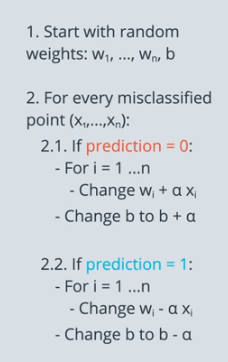
\includegraphics[width=0.2\textwidth,height=0.2\textheight,keepaspectratio]{images/perceotron_algorithm.png}
    \captionsetup{justification=centering}
    \caption{The perceptron Pseudocode}
    \label{fig:f16}
\end{figure}
  
Let's look more carefully at the model presented in Fig. \ref{fig:f3} for accepting and rejecting students. Imagine that the student four got nine in the test but only one on the grades. According to the model this student gets accepted since it's placed in the positive region of this line. Nevertheless, this is not accurate. A more precise model is presented in Fig. \ref{fig:f7}, however, this is non-linear separable. To create an accurate model a different boundary should be used, two lines, a circle or a polynomial function are just few examples of this. Unfortunately, \textbf{the perceptron algorithm won't work well for non-linear problems}. Therefore, something more complex needs to be applied to redefine the simple perceptron algorithm for a line in a way that it'll generalize to other types of curves. Nevertheless, this problem will be tackle later.

\begin{figure}[ht]
    \centering
    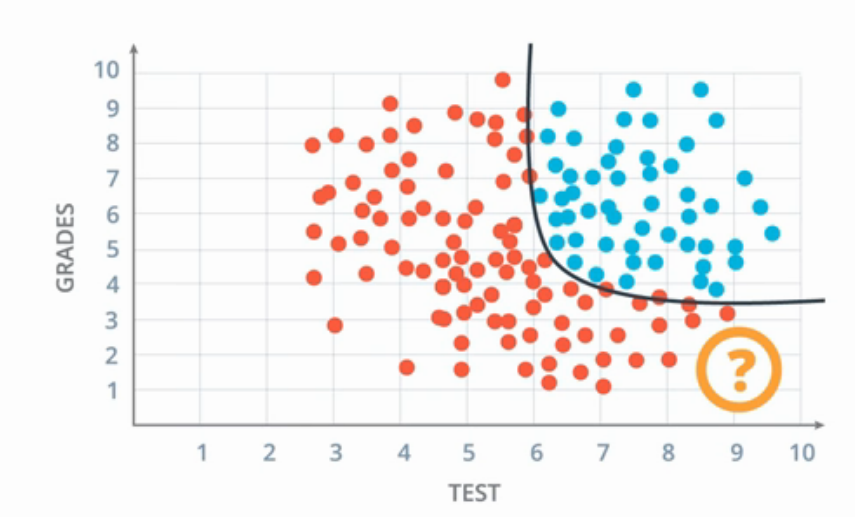
\includegraphics[width=0.35\textwidth,height=0.35\textheight,keepaspectratio]{images/non_linear.png}
    \captionsetup{justification=centering}
    \caption{Non-linear area}
    \label{fig:f17}
\end{figure}

To tackle Deep learning problems, it is necessary to introduce the concept of \textbf{Error function}. This is simply something that tells how far is the current model from the solution. An example of a simple error function used in the last example would be a function that tells how far is a point from its good classification region (distance).

\textbf{Gradient descent} is a method to reduce the error of a problem and find the global optimum using known metrics. This algorithm calculates the error and then takes a step towards the direction that minimizes the error in a problem. As an example for the Fig. \ref{fig:f13} it is possible to construct an error function which consists of the sum of the distance of the points to the boundary lines, where the misclassified points have a big penalty while the well classifies have a low penalty. This function can be used to guide the boundary line towards a direction that minimizes the error and thus, find the optimal model to solve the problem. \textbf{Note:} the error function should be differentiable and continuous. 

Recall that a discrete prediction might be something like a 1 or zero, whereas a continuous prediction would be a number, normally between zero and one. As an example, see the  Fig. \ref{fig:f18} where we have students with discrete predictions (left) and continuous predictions(right). In the discrete plot, the algorithm will tell if a student is accepted (1 - blue) or rejected (0 - red). In the continuous plot, the farther the point is from the black line, the more drastic these probabilities are. Points that are well into the blue area get very high probabilities And points that are well into the red region are given very low probabilities. The points over the line are all given a 50\% probability. The probability is a function of the distance from the line.

\begin{figure}[ht]
    \centering
    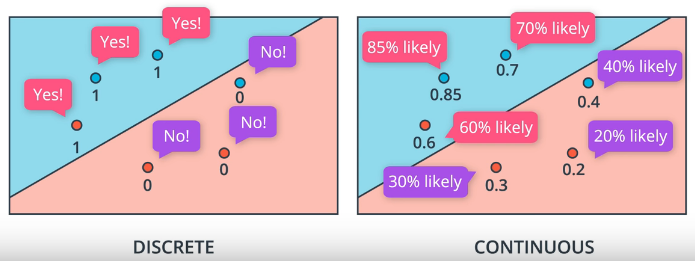
\includegraphics[width=0.5\textwidth,height=0.5\textheight,keepaspectratio]{images/discrete_continuous.png}
    \captionsetup{justification=centering}
    \caption{Discrete and continuous predictions}
    \label{fig:f18}
\end{figure}

To change from discrete to continuous predictions it is necessary to use a \textbf{Sigmoid function} (Fig. \ref{fig:f19}) instead of a unitary step as the activation function. This activation will guarantee a continuous functions instead of a discrete one, allowing the usage of gradient descent techniques. The equation of the Sigmoid function is given in the Equation \eqref{eq:8}. Before the model consisted of a line with a positive region and a negative region. With the Sigmoid function now it consists of an entire probability space for each point in the plane.

\begin{figure}[ht]
    \centering
    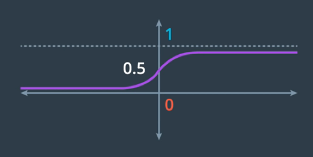
\includegraphics[width=0.35\textwidth,height=0.35\textheight,keepaspectratio]{images/sigmoid.png}
    \captionsetup{justification=centering}
    \caption{Sigmoid function}
    \label{fig:f19}
\end{figure}

\begin{equation}
\label{eq:8}
\sigma(x) = \frac{1}{1 - e^{-x}} 
\end{equation}  

Using the Sigmoid function as the activation function to predict \(\hat{y}\), the output of the perceptron will be as follows Eq. \eqref{eq:9}. The simple perceptron seen in Fig. \ref{fig:f8} with a step function can be modified as shown by Fig. \ref{fig:f20} to work with a Sigmoid function as the activation function.  Before it used to say the student got accepted or not, with the Sigmoid function it says the probability of the student got accepted is this much.

\begin{equation}
\label{eq:9}
\hat{y} = \sigma(Wx + b)
\end{equation} 

\begin{figure}[ht]
    \centering
    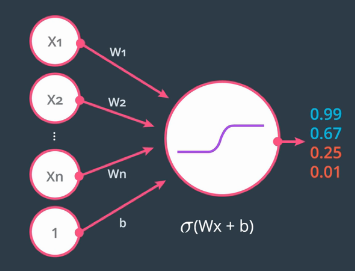
\includegraphics[width=0.30\textwidth,height=0.30\textheight,keepaspectratio]{images/perceptron_sigmoid.png}
    \captionsetup{justification=centering}
    \caption{Simple perceptron with a sigmoid activation function}
    \label{fig:f20}
\end{figure}

\textbf{The softmax function} is used when the problem has more than two classes and gives a probability of zero or one being zero as "not the class" and one as "object of this class". This is the equivalent of the sigmoid activation function, but when the problem has 3 or more classes. It is important to point out that the probability of all classes must add to one and there could not be any negative probability. To define the Softmax function let's imagine that there are N classes and a linear model that gives the following scores \( Z_1, Z_2, \dots Z_n\), each score for each of the classes in the problem. The softmax probability of the class \(Z_i\) is defined by the equation \eqref{eq:10}.

\begin{equation}
\label{eq:10}
P(\text{class i}) = \frac{e^{Z_i}}{e^{Z_i} + \dots + e^{Z_n}}  = \frac{e^{Z_i}}{\sum_k^N e^{Z_k}}
\end{equation} 

When there are multiple output classes, it is necessary to use a specific output format called \textbf{one-hot encoding}. This format assign one variable per class and outputs a one in the specific class that is selected.  Imagine that the classes are Duck, Beaver and Walrus. Here it is necessary to assign one variable for each of the classes. In the Fig. \ref{fig:f21} That's one variable for Duck, one for Beaver and one for Walrus And, each one has its corresponding column. E.g., if the input is a duck then the variable for duck is 1 and the variables for beaver and walrus are 0.

\begin{figure}[ht]
    \centering
    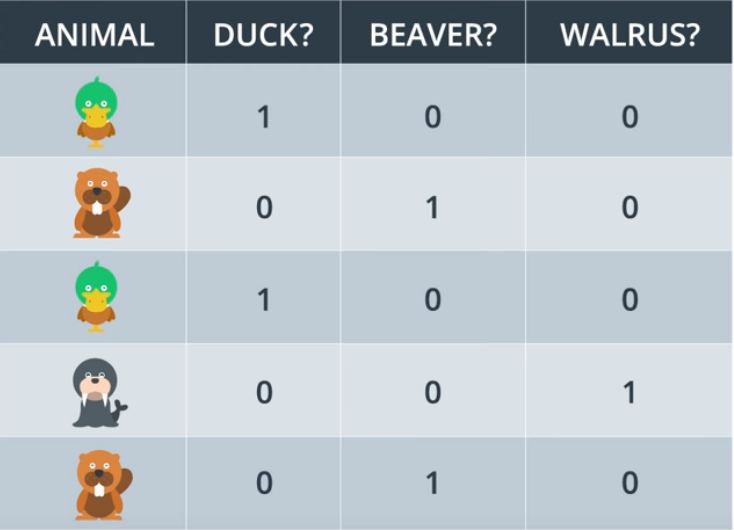
\includegraphics[width=0.45\textwidth,height=0.45\textheight,keepaspectratio]{images/one_hot.png}
    \captionsetup{justification=centering}
    \caption{One-hot encoding}
    \label{fig:f21}
\end{figure}

\textbf{Maximum likelihood} is when the model picked gives the existing labels the highest probability. Thus, by maximizing the probability, it is possible to pick the best possible model. To use an example of how maximum likelihood works, see the model presented in Fig. \ref{fig:f22}, where the value presented in each dot is the probability of being blue or red (determined by the color of the number). To determine which model is better, it is necessary to compute the probability of the four points, this probability is called the \textbf{probability space} and will tell if the points are of the colors that they actually are. For the left model, the probability space is \(0.1 x 0.6 x 0.7 x 0.2 = 0.0084\) which is a very small value, whereas for the right model the probability space is \(0.7 x 0.8 x 0.9 x 0.6 = 0.3024\). This value means that the probability that the points of the left model are of these colors is 0.0084 and the right model is 0.3024, therefore, it confirms that the model on the right is better because it makes the arrangement of the points much more likely to have those colors. If the likelihood or probability space of the model is improved, hence the model will be better/

\begin{figure}[ht]
    \centering
    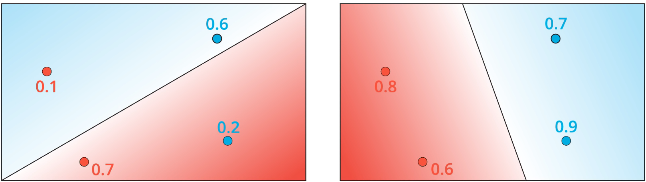
\includegraphics[width=0.45\textwidth,height=0.45\textheight,keepaspectratio]{images/likelihood.png}
    \captionsetup{justification=centering}
    \caption{Maximum likelihood example}
    \label{fig:f22}
\end{figure}

Maximizing the probability is equivalent to minimizing the error function and thus, improve the model. To start with this, it is important to transform the products of the probability of the whole arrangement into a sum, this is possible by passing the individual probabilities in a logarithmic function owing to \(\ln{ab} = \ln{a} + \ln{b}\). Applying logarithms to the example shown in Fig. \ref{fig:f22}, and taking into account that the logarithm of a number between zero and one is always negative, it is possible to use the sum of the negatives of the logarithms instead of a positive sum. Therefore, the model of the left gives \(\ln{0.6} - \ln{0.2} - \ln{0.1} - \ln{0.7} = 4.8\) ad \(\ln{0.8} - \ln{0.6} - \ln{0.7} - \ln{0.9} = 1.2\). This concepts of the negative sum of logarithms is called \textbf{Cross-entropy} and it gives a high value for bad models (left) and low values for good models (right) which is a measurement of how good the model is. 

Using the Cross Entropy concept in the last example the result can be seen in Fig. \ref{fig:f23}. The Cross-Entropy of misclassified points have really high values whereas the well classified points have low values. Thus it is possible to think of the negatives of these logarithms as errors at each point. Points that are correctly classified will have small errors and points that are misclassified will have large errors. With this it is feasible to concluded that the cross-entropy will tell us if a model is good or bad. The goal has changed from maximizing a probability to minimizing a cross-entropy in order to get from the model in left to the model in the right in Fig. \ref{fig:f23}. \textbf{The error-function is the cross-entropy}.

\begin{figure}[ht]
    \centering
    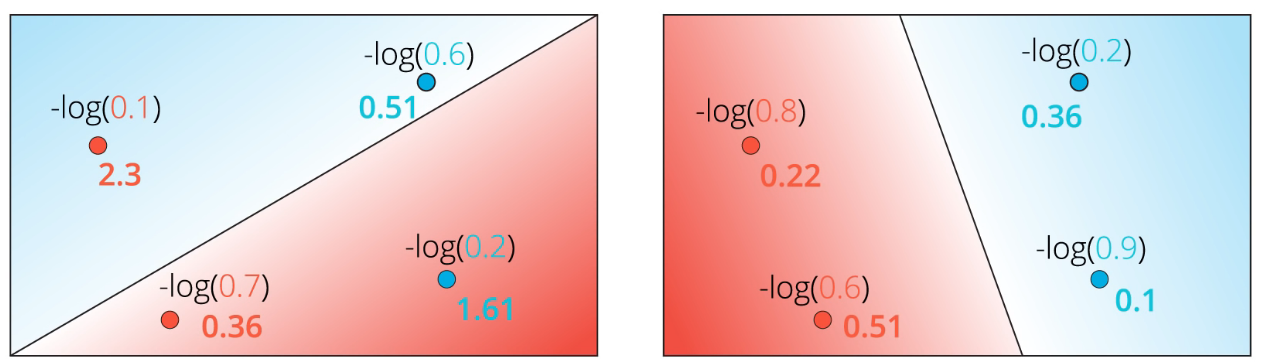
\includegraphics[width=0.45\textwidth,height=0.45\textheight,keepaspectratio]{images/cross_entrophy.png}
    \captionsetup{justification=centering}
    \caption{Using Cross Entropy example}
    \label{fig:f23}
\end{figure}

The formula of the Cross-entropy is given in Eq. \eqref{eq:11} where \(y_i\) is the true label of the class being 1 for blue and 0 for red (see Fig. \ref{fig:f23}). If \(y_i\) is one, then the probability is \(p_i\), otherwise the probability will be \((1 - p_i)\) which is the probability for \(y_i = 0\).

\begin{equation}
\label{eq:11}
Cross-Entropy = - \sum_{i = 1}^m y_i \ln{p_i} + (1 - y_i) \ln{(1 - p_i)}
\end{equation} 

When there are more than two classes, the equation of cross-entropy has to change and find a different expressions to compute these probabilities. In the Fig. \ref{fig:f24} it is possible to see an example of this. There are three different animal classes and three different "doors". Recall that the probability of each column or door must add up to 1. E.g, the probability to obtain a duck from the door two is equals to \(P_{12}\).

\begin{figure}[ht]
    \centering
    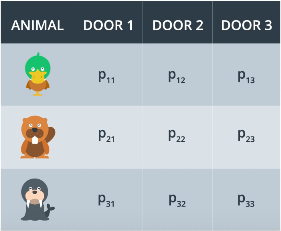
\includegraphics[width=0.3\textwidth,height=0.3\textheight,keepaspectratio]{images/multiple_classes.png}
    \captionsetup{justification=centering}
    \caption{Multiple classes example}
    \label{fig:f24}
\end{figure}

Expressing this mathematically as shown by Fig. \ref{fig:f25} the output \(y_{ij}\) is one if a specific class is obtained from the door \(j\). Therefore, the equation for \textbf{multi-class entropy} is given by Eq. \eqref{eq:12} where m is the number of classes.

\begin{figure}[ht]
    \centering
    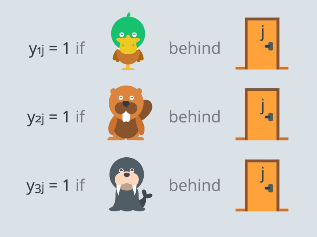
\includegraphics[width=0.3\textwidth,height=0.3\textheight,keepaspectratio]{images/multiple_notation.png}
    \captionsetup{justification=centering}
    \caption{Multiple classes notation}
    \label{fig:f25}
\end{figure}

\begin{equation}
\label{eq:12}
Cross-Entropy = - \sum_{i = 1}^m \sum_{j=1}^n y_{ij}  \ln{p_{ij}}
\end{equation} 

Recall the Fig. \ref{fig:f23} where there are two models and the cross-entrophy was calculated. The cross-entropy calculation gave 4.8 for the left model and 1.2 for the right model. The expression given in Eq \eqref{eq:13} can be used as an error given the following data. Consider that if \(y = 1\) which is blue class then \(P(blue) = \hat{y}\), therefore \(Error = -\ln{(\hat{y})}\). Now, analizing the red classification if \(y = 0\) (red class) then \(P(red) = 1 - P(blue) = 1 - \hat{y}\), thus the error for the red class would be \(Error = -\ln{(1 - \hat{y})}\).

The last analizis leads to the next Error expression.

\begin{equation}
\label{eq:13}
Error = -(1 - y)(\ln{(1 - \hat{y})} - y\ln{(\hat{y})}
\end{equation} 

The expression given in Eq \eqref{eq:13} can be used as an error, so changing the notation the error function and averaging by m gives the Equation in \eqref{eq:14}.

\begin{equation}
\label{eq:14}
Error = - \frac{1}{m} \sum_{i=1}^m (1 - y_i) (\ln{(1 - \hat{y})}) + y_i\ln{(\hat{y})}
\end{equation} 

Where \(\hat{y}\) is the output of the network. Transforming \(\hat{y}\) in terms of Eq. \eqref{eq:9}, the Eq. \eqref{eq:14} will be as follows (Eq. \eqref{eq:15}).

\begin{equation}
\label{eq:15}
E(W,b) = - \frac{1}{m} \sum_{i=1}^m (1 - y_i) (\ln{(1 - \sigma(Wx^{(i)} + b))}) + y_i\ln{(\sigma(Wx^{(i)} + b))}
\end{equation} 

The goal is to minimize the Error function given by Eq. \eqref{eq:15}. Now if there are more than two classes, the only change would be to add the additional summation as shown by Eq. \eqref{eq:12} to the error function. The Error function for more than one class is given as follows Eq. \eqref{eq:16}.

\begin{equation}
\label{eq:16}
E(W,b) = - \frac{1}{m} \sum_{i=1}^m \sum_{j=1}^n y_{ij}\ln{(\sigma(Wx^{(ij)} + b))} 
\end{equation} 

Minimizing this error leads to an algorithm called \textbf{Logistic regression } which is very popular in Machine Learning and AI. The procedure of this algorithm is given as follows:

\begin{itemize}
  \item Take the data
  \item Pick a random model
  \item Calculate the error
  \item Minimize the error, and obtain a better model
\end{itemize}

Now, to accomplish the last step of the items and minimize the error it is necessary to use the gradient descent algorithm which will allow the minimization of the error and pass from \(E(W,b)\) to \(E(W',b')\) where \(E(W',b') < E(W,b)\).

Imagine a person somewhere in a Mount where the objective is to go down Fig. \ref{fig:f26}. The inputs of the functions are \(W_1\) and \(W_2\), the error function is given by E. The gradient of E (\(\nabla E\)) is given by the vector sum of the partial derivatives \(\frac{\partial E}{\partial w_1}\) and \(\frac{\partial E}{\partial w_2}\). This gradient actually tells the direction the person has to move if he want to increase the error function the most (go up). Thus, taking the negative of the gradient,leads to decrease the error function the most. Taking the negative direction of the gradient will eventually take the person to the bottom of the mountain and decrease the error to a minimum expression. Additinally, taking steps in the direction of the negative of the gradient will also change the Weights and Bias values. This is basically the \textbf{gradient descent} algorithm. 

\begin{figure}[ht]
    \centering
    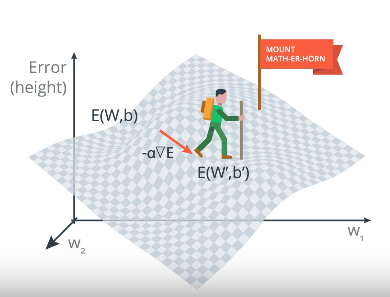
\includegraphics[width=0.45\textwidth,height=0.45\textheight,keepaspectratio]{images/gradient.png}
    \captionsetup{justification=centering}
    \caption{Gradient descent example}
    \label{fig:f26}
\end{figure}

To calculate the gradient the next equations are used. First of all the initial prediction is given by the next equation.

\[\hat{y} = \sigma(Wx + b)\]

Writing the prediction in terms of the vectors W and B gives.

\[\hat{y} = \sigma(W_1X_1 + \dots + W_nX_n + b)\]

The gradient of the error function is the vector formed by the partial derivative of the error function with respect to the weights and the bias.

\[\nabla E = (\frac{\partial E}{\partial W_1}, \dots, \frac{\partial E}{\partial W_2}, \frac{\partial E}{\partial b})\]

To avoid any drastic changes, a small learning rate alpha is introduced.

\[\alpha = 0.1\]

Multiplying the gradient by the learning rate \(\alpha\) and taking a step is the negative direction of the gradient is the same thing as updating the weights and the bias as follows, where the weight \(W_i\) will now become \(W_i'\)

\[w_i' \leftarrow w_i - \alpha \frac{\partial E}{\partial W_i}\]

The bias will now become:

\[b_i' \leftarrow b - \alpha \frac{\partial E}{\partial b}\]

The full derivation of the gradient descent is as follows. First of all, it is necessary to compute the derivative of the sigmoid function (supposing that this is our activation function) which is Eq. \eqref{eq:17}

\begin{equation}
\label{eq:17}
\sigma'(x) = \sigma(x)(1 - \sigma(x)) 
\end{equation} 

The demonstration of the last result is shown below.

\[\sigma'(x) = \frac{\partial}{\partial x} \frac{1}{1 + e ^{-x}}\]
\[\sigma'(x) = \frac{e ^{-x}}{(1 + e ^{-x})^2}\]
\[\sigma'(x) = \frac{1}{1 + e ^{-x}} \frac{e ^{-x}}{1 + e ^{-x}}\]
\[\sigma'(x) = \sigma(x)(1 - \sigma(x)) \]

Recall the Fig. \ref{fig:f23} where there are m points labeled \(X^{(1)}, X^{(2)}, \dots, X^{(m)} \), thus the error equation would be Eq. \eqref{eq:14}

\[E = - \frac{1}{m} \sum_{i=1}^m y_i\ln{(\hat{y})} + (1 - y_i) (\ln{(1 - \hat{y})})\]

The goal is to calculate \(\nabla E\), at a point \(x = (x_1, x_2,\dots,x_n)\)), given by the partial derivatives

\[\nabla E = \frac{\partial E}{\partial w_1}, \dots, \frac{\partial E}{\partial w_n}, \frac{\partial E}{\partial b}\]

To simplify the calculations, think of the error that each point produces, and calculate the derivative of this error. The total error, then, is the average of the errors at all the points. The error produced by each point is:

\[ E = -y_i\ln{(\hat{y})} - (1 - y_i) (\ln{(1 - \hat{y})})\]

In order to calculate the derivative of this error with respect to the weights, first calculate \(\frac{\partial \hat{y}}{\partial w_j}\), recalling that \(\hat{y} = \sigma(Wx + b) = \sigma(\theta)\). The 

\[\frac{\partial \hat{y}}{\partial w_j} = \frac{\partial}{\partial w_j} \sigma(Wx + b) \]
\[\frac{\partial \hat{y}}{\partial w_j} = \sigma(Wx + b)(1 - \sigma(Wx + b)) \frac{\partial}{\partial w_j}Wx + b \]
\[\frac{\partial \hat{y}}{\partial w_j} = \hat{y}(1 - \hat{y}) \frac{\partial}{\partial w_j}(w_1x_1+\dots+w_ix_i+\dots+w_nx_n, + b) \]
\[\frac{\partial \hat{y}}{\partial w_j} = \hat{y}(1 - \hat{y}) x_i \]

The last equality is because the only term in the sum which is not a constant with respect to \(w_j\) is \( w_jx_j\) which clearly has derivative \(x_j\).

Reall that the gradient descent is based on the chain rule, which would be the one described in Eq. \eqref{eq:18} where \(\theta = Wx + b\)

\begin{equation}
\label{eq:18}
\frac{\partial E}{\partial w_j} = \frac{\partial E}{\partial \hat{y}} \frac{\partial \hat{y}}{\partial w_j} =  \frac{\partial E}{\partial \hat{y}} \frac{\partial \sigma(\theta)}{\partial \theta} \frac{\partial \theta}{\partial w_j}
\end{equation} 

Now, To calculate the derivative of the error \(E\) at a point \(x\) with respect to the weight \(w_j\) is as follows.

\[\frac{\partial E}{\partial w_j} = \frac{\partial}{\partial w_j} [-y\ln{(\hat{y})} - (1 - y) (\ln{(1 - \hat{y})})] \]
\[\frac{\partial E}{\partial w_j} = -y \frac{\partial}{\partial w_j} \ln{(\hat{y})} - (1 - y) \frac{\partial}{\partial w_j} \ln{(1 - \hat{y})} \]
\[\frac{\partial E}{\partial w_j} = -y \frac{1}{\hat{y}} \frac{\partial}{\partial w_i} \hat{y} - (1 - y) \frac{1}{1 - \hat{y}} \frac{\partial}{\partial w_i} (1 - \hat{y}) \]
\[\frac{\partial E}{\partial w_j} = -y \frac{1}{\hat{y}} \hat{y}(1 - \hat{y}) x_i - (1 - y) \frac{1}{1 - \hat{y}} (-1)(\hat{y}(1 - \hat{y}) x_i) \]
\[\frac{\partial E}{\partial w_j} = -y (1 - \hat{y}) x_i + (1 - y)\hat{y}x_i \]
\[\frac{\partial E}{\partial w_j} = -(y - \hat{y})x_i \]

The Eq. \eqref{eq:19} gives the gradient of the weights.

\begin{equation}
\label{eq:19}
\frac{\partial E}{\partial w_j} = -(y - \hat{y})x_i
\end{equation} 

Similarly, the result for the bias is Eq. \eqref{eq:20}

\[ \frac{\partial E}{\partial b} = \frac{\partial E}{\partial \hat{y}} \frac{\partial \hat{y}}{\partial b} =  \frac{\partial E}{\partial \hat{y}} \frac{\partial \sigma(\theta)}{\partial \theta} \frac{\partial \theta}{\partial b} \]

\begin{equation}
\label{eq:20}
\frac{\partial E}{\partial b} = -(y - \hat{y})
\end{equation} 

In summary the gradient is:

\[\nabla E = -(y - \hat{y})(x_1,\dots ,x_n,1)\]

Therefore, a small gradient means that it changes the coordinates by a little bit, and a large gradient means it changes the coordinates by a lot.

\textbf{The gradient descent step} rule to update the weights is as follows Eq. \eqref{eq:21}

\begin{equation}
\label{eq:21}
w_i' \leftarrow w_i - \alpha-(y - \hat{y})x_i = w_i + \alpha(y - \hat{y})x_i
\end{equation}

To update the bias the equation is the next:

\begin{equation}
\label{eq:22}
b' \leftarrow b + \alpha(y - \hat{y})
\end{equation}

Note: Since the average of the errors were taken, the term added should be \(\frac{1}{m}*\alpha\) instead of \(\alpha\) but as \(\alpha\) is a constant, then in order to simplify calculations, it is possible to take \(\frac{1}{m}*\alpha\) to be the learning rate, and abuse the notation by just calling it \(\alpha\).

The gradient descent algorithm is given in the Fig. \ref{fig:f27}.

\begin{figure}[ht]
    \centering
    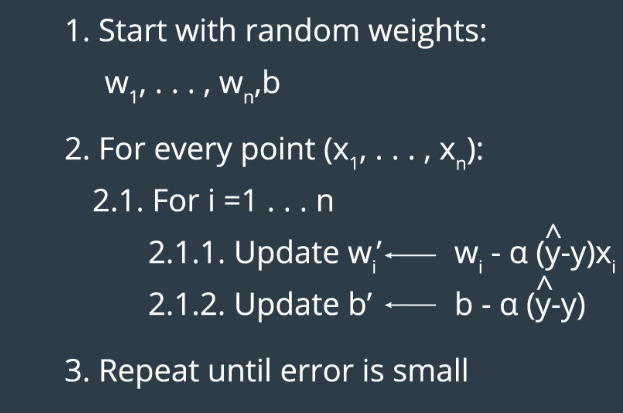
\includegraphics[width=0.45\textwidth,height=0.45\textheight,keepaspectratio]{images/gradient_algorithm.png}
    \captionsetup{justification=centering}
    \caption{Gradient descent algorithm}
    \label{fig:f27}
\end{figure}

Recall the problem presented in Fig. \ref{fig:f17}, where the problem was not linear separable. To tackle this problem it is necessary to generate a non-linear probability distribution which accurately classified the blue and red points.
\textbf{Nonlinear models} can be generated by the combination of two linear models. To make it possible, see the Fig. \ref{fig:f28} where in the left are the linear models to be combined, in the middle is the computation of one single point of the model and finally, the result after the application of the sigmoid function. 

\begin{figure}[ht]
    \centering
    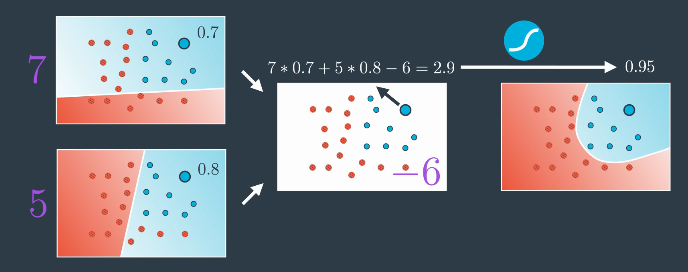
\includegraphics[width=0.6\textwidth,height=0.6\textheight,keepaspectratio]{images/adding_perceptrons.png}
    \captionsetup{justification=centering}
    \caption{Adding two perceptrons}
    \label{fig:f28}
\end{figure}

Imagine taking the point highlighted in the Fig. \ref{fig:f28}, which has a probability of \(0.7\) in the first linear model and \(0.8\) in the second model. Adding some weights to this model is possible and hence, modify its influence on the result. In this particular example, the first model has a weight of \(7\) and the second of \(5\). Therefore, the linear equation for the point highlighted gives the next linear combination \(7*0.7 + 5*0.8 - 6 = 2.9\), where \(b = -0.6\) and \(P(x_i) = 2.9\) is the probability of that point being blue. The final step is apply the sigmoid function to approximate the probability to 1, with this the final result of the point is \(0.95\) which is the probability of being blue in the resulting probability space. 

The overall steps to generate nonlinear models with linear ones is:

\begin{itemize}
  \item Calculate the probability for one of the points
  \item calculate the probability for the other models
  \item Add the probabilities times its weights and bias
  \item Apply the sigmoid function
\end{itemize}

This might result very simple but this is at the heart of how neural networks work.

The following image (Fig. \ref{fig:f29}) shows the representation of the example in Fig. \ref{fig:f28} but as a combination of nodes and weights. This representation clearly shows how the perceptrons are combined to produce and new non-linear output.

\begin{figure}[ht]
    \centering
    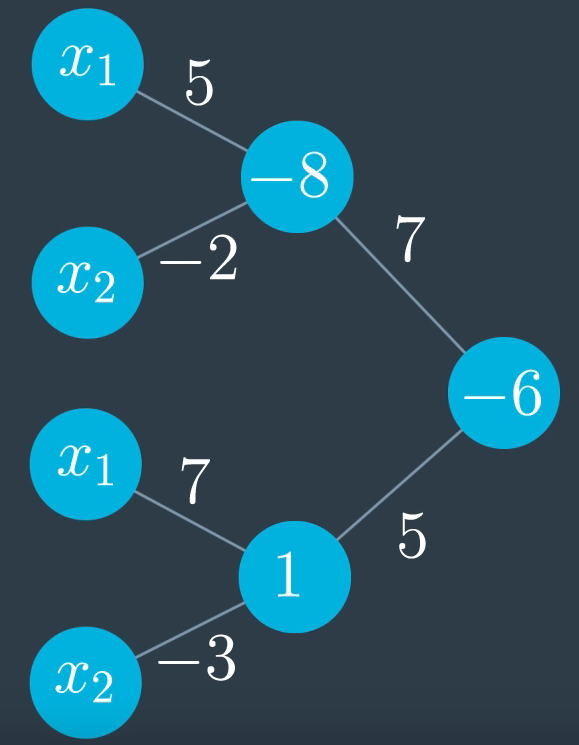
\includegraphics[width=0.25\textwidth,height=0.25\textheight,keepaspectratio]{images/adding_perceptrons_2.png}
    \captionsetup{justification=centering}
    \caption{The perceptrons as a neural network}
    \label{fig:f29}
\end{figure}

The Fig. \ref{fig:f30} is an even more simplified representation of Fig. \ref{fig:f29} where all the input nodes connects with the middle nodes and these connects to a unique output. Additionally, this representation has the bias in each layer and shows the activation function needed (sigmoid) to obtain a non-linear function in the input.

\begin{figure}[ht]
    \centering
    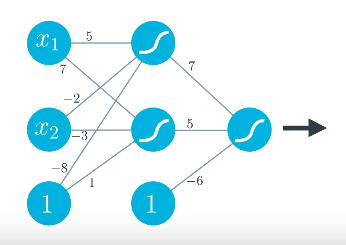
\includegraphics[width=0.4\textwidth,height=0.4\textheight,keepaspectratio]{images/adding_perceptrons_3.png}
    \captionsetup{justification=centering}
    \caption{The simplified representation of multiple perceptrons in a neural network}
    \label{fig:f30}
\end{figure}

Neural networks have a certain special \textbf{architecture} with layers. The first layer is called the input layer, which contains the inputs. The next layer is called the hidden layer, which is a set of linear models created with this first input layer. Then the final layer is called the output layer, where the linear models get combined to obtain a nonlinear model. It is possible to create different architectures with various inputs, hidden layers or outputs. 

\textbf{The number of input} noted defined the dimension of the problem. Two input nodes turn the second layer into a two-dimensional representation whereas three inputs generates three dimensional representations or planes in the hidden layer. 

\textbf{Adding hidden layers} increase the amount of representations that can be generated with the neural network and create more complex boundaries than with only two layers. 

Finally, \textbf{adding more outputs} creates multiple categories and opens the possiblity to classify different things like cat, dogs or birds. \textbf{Note:} if the model has multiple outputs, it is necessary to change the activation in the last function for a Softmax activation function and add as many outputs as classes are present in the problem. This activation function will guarantee a probability distribution in the last layer and will show which of the classes is the selected one with the highest probability.

\textbf{Feedforward} is the process neural networks use to turn the input into an output, passing the whole data throughout the network. In the Fig. \ref{fig:f31} is an example of this with a network with two input layers, two hidden units and one output. The Weights \(W^{1}\) corresponds to the weights between the input layer and the hidden layer, for a matter of simplicity, the bias was added to this set of weights. Similarly, the weights \(W^{2}\) are between the hidden layer and the output layer. Mathematically, the feedforward process can be expressed as shown by Eq. \eqref{eq:23}. \textbf{Note:} the bias are now denoted as \(W_{31}^{(1)}, W_{32}^{(1)}, W_{31}^{(2)}\)

\begin{equation}
\label{eq:23}
\hat{y} = \sigma(\sigma (\begin{bmatrix}
           x_{1} \\
           x_{2} \\
           1
         \end{bmatrix} \cdot \begin{pmatrix}
                                W_{11}^{(1)} & W_{12}^{(1)} \\
                                W_{21}^{(1)} & W_{22}^{(1)} \\
                                W_{31}^{(1)} & W_{32}^{(1)}
                                \end{pmatrix} ) \cdot \begin{bmatrix}
                                                           W_{11}^{(2)} \\
                                                           W_{21}^{(2)} \\
                                                           W_{31}^{(2)}
                                                         \end{bmatrix})
\end{equation}

\begin{figure}[ht]
    \centering
    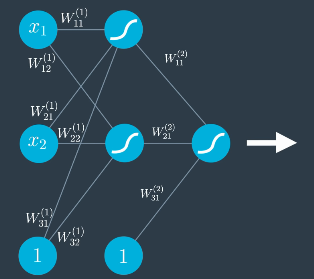
\includegraphics[width=0.4\textwidth,height=0.4\textheight,keepaspectratio]{images/feedforward.png}
    \captionsetup{justification=centering}
    \caption{Feedforward in a neural network}
    \label{fig:f31}
\end{figure}

Equation \eqref{eq:23} can be simplied into Eq. \eqref{eq:24}. As a rule of thumb, feedforward takes the input vector and then apply a sequence of linear models and sigmoid functions or whatever activation function is used in the network. The feedforward process is used to obtain the prediction from the input vector. These steps can be extended into more deep networks as the procedure is always the same.

\begin{equation}
\label{eq:24}
\hat{y} = \sigma(\sigma(W^{(1)} \cdot X) \cdot W^{(2)})
\end{equation}

The error function for a multi-layer perceptron is exactly the same used for the perceptron algorithm which is Eq. \eqref{eq:14} or the Cross-entropy. Similarly, \(\hat{y} = \sigma(Wx + b)\) but for a neural netowrk with multiple layers, the only difference is that \(\hat{y}\) is more complex and is a combination of multiplications and sigmoid functions as shown here \[\hat{y} = \sigma W^{(3)} \cdot \sigma W^{(2)} \cdot \sigma W^{(1)} \cdot X \]

\textbf{Backpropagation} is the method used to train multilayer perceptrons or deep neural networks. At a glance, this is the opposite process of feeding forward a neural network, to propagate the error backwards and correct the value of the weights towards a good model or solution. The steps for this algorithm are:

\begin{itemize}
  \item Doing a feedforward operation.
  \item Comparing the output of the model with the desired output.
  \item Calculating the error.
  \item Running the feedforward operation backwards (backpropagation) to spread the error to each of the weights.
  \item Use this to update the weights, and get a better model.
  \item Continue this until we have a model that is good.
\end{itemize}

To start, recall that for the perceptron algorithm, the prediction was given by Eq. \eqref{eq:9}, the error is the cross-entropy (Eq. \eqref{eq:14}) and the objective is to calculate the gradient of the error function \(\nabla E = \frac{\partial E}{\partial w_1}, \dots, \frac{\partial E}{\partial w_n}, \frac{\partial E}{\partial b}\).
    
For a multilayer perceptron as the one presented in Fig. \ref{fig:f31}, The prediction is given by Eq. \eqref{eq:25}, the error function is exactly the same as in the perceptron algorithm Eq. \eqref{eq:14} and the gradients of the error are the same but with way more calculations Eq. \eqref{eq:26}.
    
\begin{equation}
\label{eq:25}
\hat{y} = \sigma W^{(3)} \cdot \sigma W^{(2)} \cdot \sigma W^{(1)} \cdot X
\end{equation}

\begin{equation}
\label{eq:26}
\nabla E = (\dots, \frac{\partial E}{\partial w_j^i}, \dots)
\end{equation}
    
Writing this more formally, the prediction is a composition of matrix multiplications and sigmoid functions.

\[\hat{y} = \sigma W^{(2)} \cdot \sigma W^{(1)} \cdot x\]

Where: 

\[ W^{(1)} = \begin{pmatrix}
                                W_{11}^{(1)} & W_{12}^{(1)} \\
                                W_{21}^{(1)} & W_{22}^{(1)} \\
                                W_{31}^{(1)} & W_{32}^{(1)}
                                \end{pmatrix} \]

\[ W^{(2)} = \begin{bmatrix}
               W_{11}^{(2)} \\
               W_{21}^{(2)} \\
               W_{31}^{(2)}
             \end{bmatrix}\]
                                
With a gradient that can be formalized as (in reality \(\nabla E\) is a long vector: 

\[ \nabla E = \begin{pmatrix}
                                \frac{\partial E}{\partial W_{11}^{(1)}} & \frac{\partial E}{\partial W_{12}^{(1)}} & \frac{\partial E}{\partial W_{11}^{(2)}} \\
                                \frac{\partial E}{\partial W_{21}^{(1)}} & \frac{\partial E}{\partial W_{22}^{(1)}} & \frac{\partial E}{\partial W_{11}^{(2)}} \\
                                \frac{\partial E}{\partial W_{31}^{(1)}} & \frac{\partial E}{\partial W_{32}^{(1)}} & \frac{\partial E}{\partial W_{11}^{(2)}} 
                                \end{pmatrix} \]
                                
The update step for the backpropagation would be Eq. \eqref{eq:27}:

\begin{equation}
\label{eq:27}
W_{ij}^{'k} \leftarrow W_{ij}^{k} + \alpha \frac{\partial E}{\partial W_{ij}^{(k)}}
\end{equation}

At this point is important to recall the chain rule, which is presented in the Fig. \ref{fig:f32}.

\begin{figure}[ht]
    \centering
    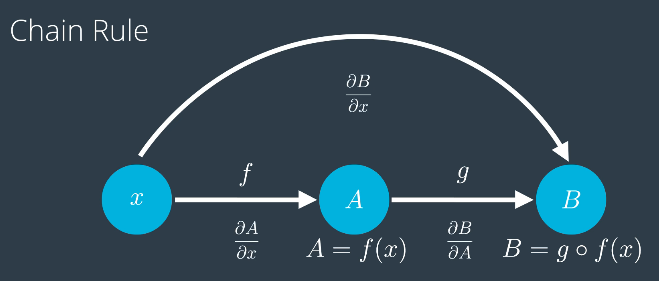
\includegraphics[width=0.5\textwidth,height=0.5\textheight,keepaspectratio]{images/chain_rule.png}
    \captionsetup{justification=centering}
    \caption{The chain rule}
    \label{fig:f32}
\end{figure}

\[\frac{\partial B}{\partial x} = \frac{\partial B}{\partial A} \frac{\partial A}{\partial x}\]

To start with the calculation of the backgropagation algorithm, the first step is to do a forward pass. The hidden nodes and the output nodes have been labeled \(h_1, h_2, h\) respectively Fig. \ref{fig:f33}. The equation of these nodes is given as follows.

\[h_1 = W_{11}^{(1)}x_1 +  W_{21}^{(1)}x_2 + W_{31}^{(1)}\]
\[h_2 = W_{12}^{(1)}x_1 +  W_{22}^{(1)}x_2 + W_{32}^{(1)}\]
\[h = W_{11}^{(2)}\sigma(h_1) + W_{21}^{(2)}\sigma(h_2) + + W_{31}^{(2)}\]

\begin{figure}[ht]
    \centering
    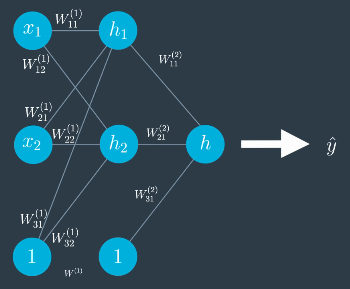
\includegraphics[width=0.4\textwidth,height=0.4\textheight,keepaspectratio]{images/feedforward_pass.png}
    \captionsetup{justification=centering}
    \caption{A feedforward pass in a MLP}
    \label{fig:f33}
\end{figure}

Similarly, the prediction is:

\[\hat{y} = \sigma(h)\]

\[\hat{y} = \sigma W^{(2)} \cdot \sigma W^{(1)} \cdot x\]

To backpropagate the error it is neccesary to calculate the gradients of the error function Eq. \eqref{eq:14} \(E(W) = - \frac{1}{m} \sum_{i=1}^m y_i\ln{(\hat{y})} + (1 - y_i) (\ln{(1 - \hat{y})})\) using the chain rule.

Since the error function is function of the prediction and the prediction is function of the weights the error function can be written as a function of the weights \(W_{ij}^{k}\) as follows:

\[E(W) = E(W_{11}^{(1)}, W_{12}^{(1)}, \dots, W_{31}^{(2)})\]

Therefore, the gradient is the vector formed by all the partial derivatives of the error function E with respect to each of the weights.

\[\nabla E = (\frac{\partial E}{\partial W_{11}^{(1)}}, \dots, \frac{\partial E}{\partial W_{31}^{(2)}})\]

With this information, it is possible to do an example and calculate the partial derivative of the error with respect to \(W_{11}^{(1)}\), this partial derivative is given by the next equation Eq. \eqref{eq:28}.

\begin{equation}
\label{eq:28}
\frac{\partial E}{\partial W_{11}^{(1)}} = \frac{\partial E}{\partial \hat{y}} \frac{\partial \hat{y}}{\partial h} \frac{\partial h}{\partial h_1} \frac{\partial h_1}{\partial W_{11}^{(1)}}
\end{equation}

Where most of the partial derivatives are already know from the perceptron algorithm Eq. \eqref{eq:19}, the only new term is: \(\frac{\partial h}{\partial h_1} \). The partial derivative of this term is giving by Eq. \eqref{eq:29} and is based on the partial derivative of the sigmoid function in Eq. \eqref{eq:17}.

\begin{equation}
\label{eq:29}
\frac{\partial h}{\partial h_1} = W_{11}^{(2)} \sigma(h_1)(1 - \sigma(h_1))
\end{equation}

This process has to be repeated for each of the weights in the neural network but it is mainly the same. If the activation function is changed, then the derivative will change. Nevertheless, the process still being the same and the gradient descent algorithm can be easy applied to different neural networks with multiple layers.

Now that the backpropagtion algorithm has been introduced, it is time to talk about testing. \textbf{Testing} is the process of evaluating a model with two different tests, the training set and the test set. In the Fig. \ref{fig:f34} the solid color points are the training set and the points with the white inside are the testing set. The training set is used to train the model without looking the test set and once the model is completely trained, the test set is used to evaluate how good the model is actually doing.

\begin{figure}[ht]
    \centering
    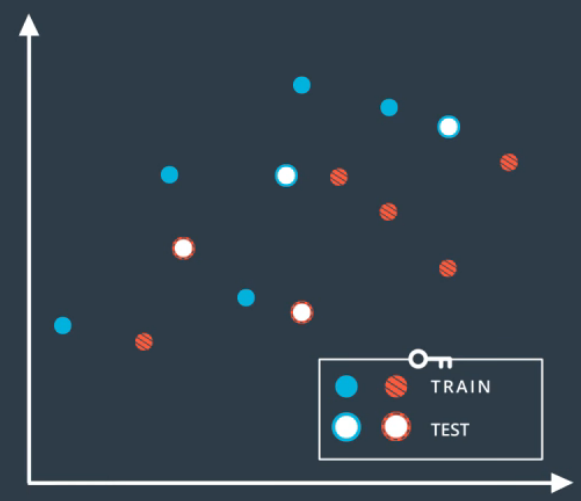
\includegraphics[width=0.4\textwidth,height=0.4\textheight,keepaspectratio]{images/testing.png}
    \captionsetup{justification=centering}
    \caption{Splitting the data into training and test sets}
    \label{fig:f34}
\end{figure}

Oversimplifying the problem means trying a solution that is too simple and won't do the job. In machine learning, this is called \textbf{underfitting}. On the other hand, when a solution is overly complicated it will probably leads to bad solutions and extra complexity when a simpler solution was just the answer. In machine learning, this is called \textbf{overfitting}. Generally, an overfitting model fits the data well but it fails when generalizing (error due to variance), whereas an underfitting model generalizes too much and tends to get the dataset bad (error due to bias).

In the Fig. \ref{fig:f35} can be seen an example of how a underfitting, just right and overfitting model looks like.

\begin{figure}[ht]
    \centering
    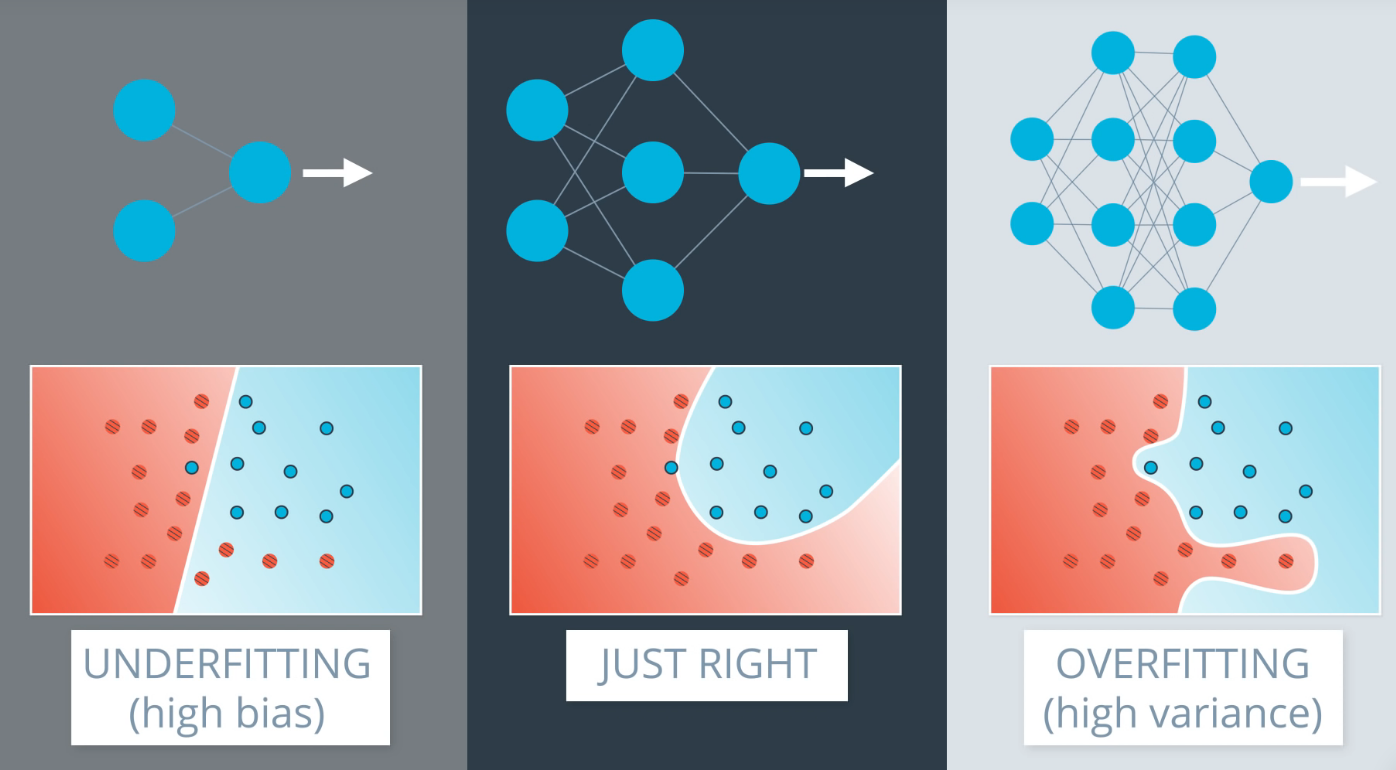
\includegraphics[width=0.6\textwidth,height=0.6\textheight,keepaspectratio]{images/under_over.png}
    \captionsetup{justification=centering}
    \caption{Underfitting and Overfitting models}
    \label{fig:f35}
\end{figure}

To try to solve this problem, it is better to always try to go for a slightly overfitting model. The idea is to approach as close as possible to the solution and then use some techniques to avoid overfitting.

One technique to solve the overfitting issue is called \textbf{early stopping}, and this is presented in Fig. \ref{fig:f36}. The plot is called the model complexity graph. In the Y-axis, there is a measure of the error and in the X-axis is a measure of the complexity of the model. In this case, the measure of complexity is the number of epochs. It is possible to see in the figure that in the left are high testing and training error, hence the model is underfitting. In the right, there are a high testing error and low training error, therefore the model is overfitting. Nevertheless in the middle is the right spot to obtain the best train and test error, the main idea of this plot is to determines the number of epochs needed.

\begin{figure}[ht]
    \centering
    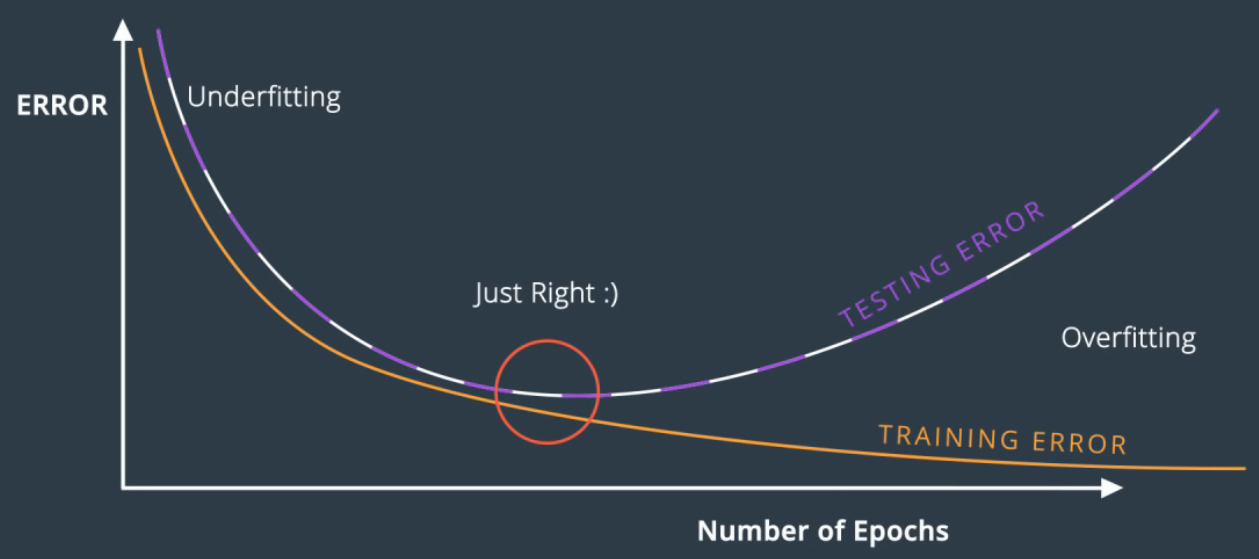
\includegraphics[width=0.5\textwidth,height=0.5\textheight,keepaspectratio]{images/early.png}
    \captionsetup{justification=centering}
    \caption{Early stopping}
    \label{fig:f36}
\end{figure}

Another technique to stop overfitting is called \textbf{regularization}. To explain it, first see the Fig. \ref{fig:f37} which presents two models with exactly the same boundary line. The only difference is that the weights of the model in the right are bigger. This difference in the weights will create a bigger estimate value which being pass through the activation function (sigmoid) will result in values very close to zero and one. However, the left model creates values between zero and one with more disparity. 

\begin{figure}[ht]
    \centering
    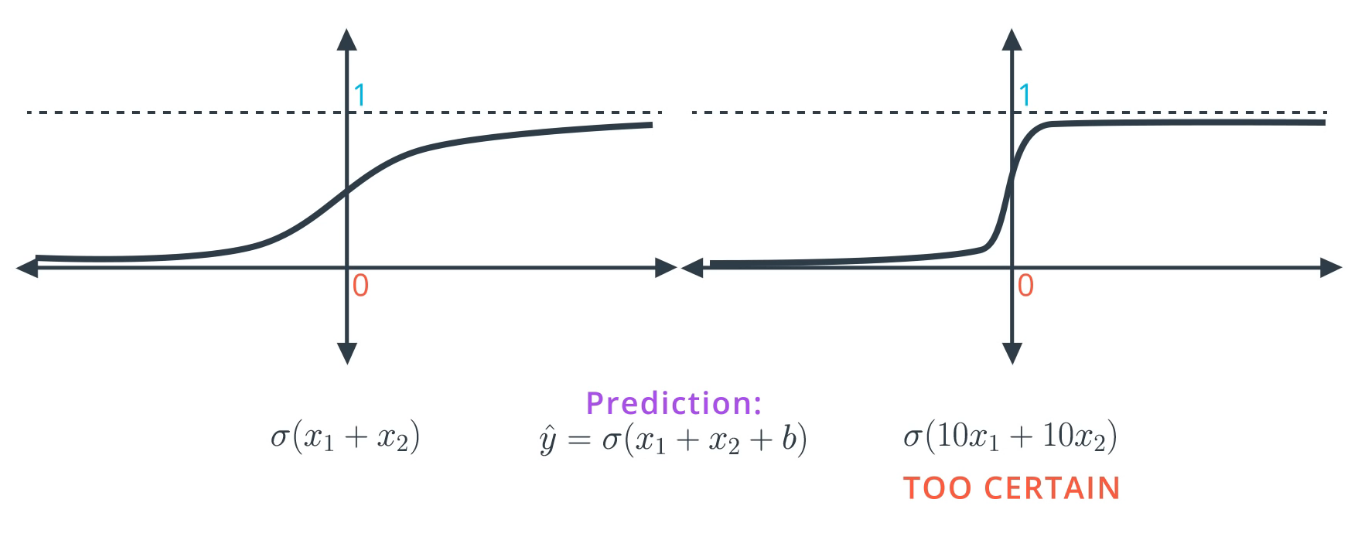
\includegraphics[width=0.6\textwidth,height=0.6\textheight,keepaspectratio]{images/regularization.png}
    \captionsetup{justification=centering}
    \caption{Early stopping}
    \label{fig:f37}
\end{figure}

This particular situation might leads the thought "The right model is the best" despite this is not true. The right model will generate a very well known problem when the gradient descent step is applied which will generate very similar values (0 or 1) when the training is being executed.

One way to prevent this is use L1 (Eq. \eqref{eq:30}) and L2 regularization (Eq. \eqref{eq:31}), which is a technique to prevent the drastic increase in the weights of the network.

\[\text{Large Coefficientes} \rightarrow \text{Overfitting}\]

\begin{equation}
\label{eq:30}
\text{L1 Error function} = - \frac{1}{m} \sum_{i=1}^m y_i\ln{(\hat{y})} + (1 - y_i) (\ln{(1 - \hat{y})} + \lambda (|w_1|+\dots+|w_n|))
\end{equation}

\begin{equation}
\label{eq:31}
\text{L2 Error function} = - \frac{1}{m} \sum_{i=1}^m y_i\ln{(\hat{y})} + (1 - y_i) (\ln{(1 - \hat{y})} + \lambda (w_1^2+\dots+w_n^2))
\end{equation}

The main difference between L1 and L2 is that L1 is good for feature selection because at the end the model end up with sparse vectors \([0,1,1,0,0]\) this means that small weights then to go to zero and big ones to one. However, L2 is normally better for training models because it tries to maintain all the weights homogeneously small \([0.2, 0.5, 0.7 ,0.9, 0.2]\).

\textbf{Dropout} is another technique to prevent overfitting. This technique randomly turn off some of the nodes and prevents the data to pass through there. In that case, the other nodes have to pick up the slack and take more part in the training. This process improves the training process a guarantee a good training of all the nodes in the network. Each epoch different nodes are turned off and this is governed by a probability, let's say \(0.2\) this probability means that per each epoch, each node has a probability of 20\% to be turned off. 



\printbibliography

\end{document}

